
%\author{Alessandro Ferreira Leite}
%\title{Estrutura de Dados \\ Estrutura de dados Linear: Pilha} 

\section{Pilha}

\begin{frame}[c]{\Large Capítulo 02 -- Pilha}


\begin{columns}
\begin{column}{.5\textwidth}
\centering
Pontos fundamentais a serem cobertos:
  \begin{enumerate}
  \item Contexto e motivação
  \item Definição
  \item Implementações
  \item Exercícios 
\end{enumerate}  

\end{column}
\begin{column}{.5\textwidth}
\centering

\includegraphics[height=5cm, width=3.5cm]{figs/fig_pilhas/pilha_livro.jpeg}
%\hspace{+0.25cm}
%\scriptsize\textcolor{red}{[Tizio, Caio et al., Nature (2006)]}
\end{column}
\end{columns}

\end{frame}
%--------------------



\subsection{Introdução} 

  \begin{frame}{Introdução}    
		\begin{itemize}
			\item Uma das estruturas de dados mais simples
			\item Embora seja uma das estrutura de dados mais utilizadas em programação
			\item A pilha se \textit{fortalece} quando combinada dentro de outras estruturas
			\begin{itemize}
			  \item Uso de pilhas na sequência de visita a nós de uma árvore
			  \item Dentro de outras estruturas como filas (depois)
			\end{itemize}
			
			\item Há uma metáfora emprestada do mundo real, que a 
			computação utiliza pilhas 
			para resolver muitos problemas de forma simplificada.
		\end{itemize}
  \end{frame}
  
  
   \begin{frame}
   \frametitle{Aplicações}


\begin{block}{Alguns exercícios são clássicos (e devemos implementá-los):}

   \begin{itemize}
     \item Balanceamento de símbolos. Exemplo: \texttt{([aaa])}
     \item Conversão da notação infixa para pós-fixa
     \item Conversão da notação infixa para in-fixa
     \item Avaliação de uma expressão pós-fixa. Exemplo: \texttt{2 3 +}
     \item Implementações de chamadas de funções (inclusive as chamadas recursivas de funções)
  %% \item Encontrar spans
     \item Armazenamento de páginas visitadas no  navegador em uma dada janela (botão \textbf{back})
     \item Sequência de comandos de um editor de texto, e depois aplique  o \textit{undo}, ou \texttt{crtl-z}
     \item Casamento de \textit{tags} in HTML e XML
     \item As teclas $\uparrow $ e $\downarrow $ na console ou terminal do Linux, duas pilhas neste caso!
     
   \end{itemize}

\end{block}
  
  
  
  \end{frame}
  
  
  
  
   \begin{frame}{Definição}
     \begin{block}{Definição}
       Um conjunto ordenado de itens no qual novos itens podem ser 
       inseridos e a partir do qual podem ser eliminados em uma 
       extremidade denominada \alert{topo} da pilha.
     \end{block}
     \pause
     \begin{block}{Definição}
       Uma seqüência de objetos, todos do mesmo tipo, sujeita às
        seguintes regras de comportamento:       
				\begin{enumerate}
					\item Sempre que solicitado a remoção de um elemento, o elemento removido é o último da seqüência.
					\item Sempre que solicitado a inserção de um novo elemento, 
					       o objeto é inserido no fim da seqüência (\alert{topo}).
				\end{enumerate}
     \end{block}  
   \end{frame}
  
   \begin{frame}{Pilha}     
			\begin{itemize}
				\item Uma pilha é um objeto dinâmico, constantemente mutável, onde elementos são inseridos e removidos.
				\item Em uma pilha, cada novo elemento é inserido no topo.
				\item Os elementos da pilha só podem ser retirado na ordem inversa à ordem em que foram inseridos				
					\begin{itemize}
						\item O primeiro que sai é o último que entrou (\textit{clássico})
						\item Por essa razão, uma pilha é dita uma estrutura 
						do tipo: \alert{LIFO}(\textit{last-in, first} ou UEPS último a entrar é o primeiro a sair.)
					\end{itemize}
			\end{itemize}
  \end{frame}
  
   \begin{frame}{Operações básicas}     
			\begin{itemize}
				\item As operações básicas que devem ser implementadas em uma estrutura do tipo pilha são:
			\end{itemize}
			\begin{table}[ht]
			  \centering
						\begin{tabular}{l|l}
						    \hline \textbf{Operação} & \textbf{Descrição} \\
						    \hline push(p, e) & empilha o elemento \textit{e}, inserindo-o no topo da pilha \textit{p}.\\
						    \hline pop(p) & desempilha o elemento do topo da pilha \textit{p}.\\
						    \hline 
						\end{tabular}
						\caption{Operações básicas da estrutura de dados pilha.}
				\end{table}
  \end{frame}
  
   \begin{frame}[c]{Exemplo} 
		   	\begin{figure}[!htpb]
				\centering
				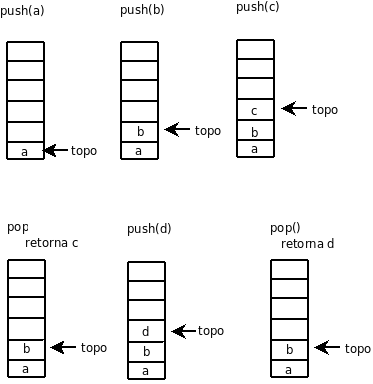
\includegraphics[width=.6\textwidth]{pilha}
			\end{figure} 
   \end{frame}
  
   \begin{frame}{Operações auxiliares}   
			\begin{itemize}
				\item Além das operações básicas, temos as operações ``\textit{auxiliares}''. São elas:
			\end{itemize}
			\begin{table}[ht]
			  \centering
						\begin{tabular}{l|l}
						    \hline \textbf{Operação} & \textbf{Descrição} \\
						    \hline create & cria uma pilha vazia.\\
						    \hline empty(p) & determina se uma pilha \textit{p} está ou não vazia.\\
						    \hline free(p) & libera o espaço ocupado na memória pela pilha \textit{p}.\\
						    \hline 
						\end{tabular}
						\caption{Operações auxiliares da estrutura de dados pilha.}
				\end{table}
  \end{frame}
  
\begin{frame}[fragile,plain]{Interface do Tipo Pilha -- Típica}
\begin{lstlisting}[language=C]
/* Definicao da estrutura */
typedef struct pilha { .... } Pilha;

/*Aloca dinamicamente ou estaticamente a estrutura pilha, 
  inicializando seus campos e retorna seu ponteiro.*/
Pilha * create(void);

/*Insere o elemento e na pilha p.*/
void push(Pilha *p, int e);

/*Retira e retorna o elemento do topo da pilha p*/
int pop(Pilha *p);

/*Informa se a pilha p esta ou nao vazia.*/
int empty(Pilha *p);
\end{lstlisting}
\end{frame}



\begin{frame}
\frametitle{Implementações} 


\begin{enumerate}

  \item Baseada em um simples vetor
    \item Baseada em um vetor dinâmico
      \item Baseada em lista encadeada
      \pause
      \item mas todas usam ponteiros!


\end{enumerate}


\end{frame}


\begin{frame}{Implementação de Pilha com Vetor}  
	\begin{itemize}
		\item Normalmente as aplicações que precisam de uma 
		estrutura pilha, é comum saber de antemão o número 
		máximo de elementos que precisam estar armazenados 
		simultaneamente na pilha.
		\item Essa estrutura de pilha tem um limite conhecido.
		\item Os elementos são armazenados em um vetor.
		\item Essa implementação é mais simples.
		\item Os elementos inseridos ocupam as primeiras posições do vetor. 
	\end{itemize}
\end{frame}

\begin{frame}{Implementação de Pilha com Vetor}  
	\begin{itemize}
		\item Seja \textit{p} uma pilha armazenada em um vetor \textit{VET} de \textit{N} elementos:		
			\begin{enumerate}
				\item O elemento vet[topo] representa o elemento do topo.
				\item A parte ocupada pela pilha é vet[0 .. topo - 1].
				\item A pilha está vazia se topo = -1.
				\item Cheia se topo = N - 1.
				\item Para desempilhar um elemento da pilha, não vazia,
				 basta $$x = vet[topo--]$$.
				\item Para empilhar um elemento na pilha, em uma pilha não cheia, 
				basta $$vet[t++] = e$$.  
			\end{enumerate}
	\end{itemize}
\end{frame}

\begin{frame}[fragile]{Implementação de Pilha com Vetor}
\begin{lstlisting}[language=C]
#define N 20 /* numero maximo de elementos*/
#include <stdio.h>
#include "pilha.h"

/*Define a estrutura da pilha*/
struct pilha{
  int topo;            /* indica o topo da pilha */
  int elementos[N];   /* elementos da pilha*/
};

Pilha* create(void){
  Pilha* p = (Pilha * ) malloc(sizeof(Pilha));
  p->topo = -1;     /* inicializa a pilha com 0 elementos */
  return p;
}	
	\end{lstlisting}  
\end{frame}

\begin{frame}[fragile,c]{Implementação de Pilha com Vetor}
\begin{itemize}
	\item Empilha um elemento na pilha
\end{itemize}
\begin{lstlisting}[language=C]
void push(Pilha *p, int e){
     if (p->topo == N - 1){ /* capacidade esgotada */
        printf("A pilha esta cheia");
        exit(1);
     }
     /* insere o elemento na proxima posicao livre */
     p->elementos[++p->topo] = e;
}	
\end{lstlisting}  
\end{frame}

%%%
\begin{frame}[fragile,c]{Implementação de Pilha com Vetor}
\begin{itemize}
	\item Desempilha um elemento da pilha
\end{itemize}
\begin{lstlisting}[language=C]
int pop(Pilha *p)
{
     int e;
     if (empty(p)){
        printf("Pilha vazia.\n");
        exit(1);             
     } 
     
     /* retira o elemento do topo */
     e = p->elementos[p->topo--];
     return e;
}	
\end{lstlisting}  
\end{frame}


\begin{frame}[fragile]{Implementação de Pilha com Vetor}
\begin{lstlisting}[language=C]
/**
 * Verifica se a pilha p esta vazia
 */
int empty(Pilha *p)
{
   return (p->t == -1);
}

\end{lstlisting}
\end{frame}

\begin{frame}{Exemplos de Uso}
\begin{itemize}
	\item Na área computacional existem diversas aplicações de pilhas. 
	\item Alguns exemplos são: caminhamento em árvores, chamadas de sub-rotinas por um compilador ou pelo sistema operacional, inversão de uma lista, avaliar expressões, entre outras.
	\item Uma das aplicações clássicas é a conversão e a avaliação de expressões algébricas. Um exemplo, é o funcionamento das calculadoras da HP, que trabalham com expressões pós-fixadas.
\end{itemize}
\end{frame}

%\begin{frame}{Avaliação de Expressões}
%	\begin{itemize}
%		\item Considere as expressões aritméticas abaixo, e imagine que é nosso objetivo avaliar se as expressões estão definidas corretamente.		
%		\begin{enumerate}
%			\item (A + B) / C
%			\item 3 +  \{[2 + (7 * 3)/5] + (C - B)\} 
%		\end{enumerate}
%	\end{itemize}
%\end{frame}
%
\begin{frame}[fragile]{Exercícios}
	\begin{enumerate}
	
	\item Os exercícios propostos no início deste capítulo (slide inicial)
	
	
		\item Escreva uma função que inverta a ordem das letras de cada palavra de uma sentença, preservando a ordem das palavras. Suponha que as palavras da sentença são separadas por espaços. A aplicação da operação à sentença \textbf{AMU MEGASNEM ATERCES}, por exemplo, deve produzir \textbf{UMA MENSAGEM SECRETA}.
		\item Implemente uma função que receba uma pilha como parâmetro e retorne o valor armazenado em seu topo, restaurando o conteúdo da pilha. Essa função deve obedecer ao protótipo: 
		\begin{verbatim}
		   char topo(Pilha* p);
		\end{verbatim} 
		\item Implemente uma função que receba duas pilhas, $p_1, p_2$, e passe todos os elementos da pilha $p_2$ para o topo da pilha $p_1$. Essa função deve obedecer ao protótipo: 
		\begin{verbatim}
		   void concatena(Pilha* p1, Pilha* p2);
		\end{verbatim} 
	\end{enumerate}
\end{frame}
